% \documentclass[aps,prl,preprint,groupedaddress]{revtex4-1}
%\documentclass[aps,prl,preprint,superscriptaddress]{revtex4-1}
\documentclass[aps,prl,reprint,superscriptaddress]{revtex4-1}
\newcommand{\SSC}{S/S_{c}}
\newcommand{\mnras}{Monthly Notices of the Royal Astronomical Society}
\newcommand{\apjs}{The Astrophysical Journal Supplement Series}
\usepackage{graphicx}

% You should use BibTeX and apsrev.bst for references
% Choosing a journal automatically selects the correct APS
% BibTeX style file (bst file), so only uncomment the line
% below if necessary.
%\bibliographystyle{apsrev4-1}

\begin{document}

% Use the \preprint command to place your local institutional report
% number in the upper righthand corner of the title page in preprint mode.
% Multiple \preprint commands are allowed.
% Use the 'preprintnumbers' class option to override journal defaults
% to display numbers if necessary
%\preprint{}

%Title of paper
\title{The Magnetorotational Instability Prefers Three Dimensions}

% repeat the \author .. \affiliation  etc. as needed
% \email, \thanks, \homepage, \altaffiliation all apply to the current
% author. Explanatory text should go in the []'s, actual e-mail
% address or url should go in the {}'s for \email and \homepage.
% Please use the appropriate macro foreach each type of information

% \affiliation command applies to all authors since the last
% \affiliation command. The \affiliation command should follow the
% other information
% \affiliation can be followed by \email, \homepage, \thanks as well.
\author{Jeffrey~S.~Oishi}
\email[]{joishi@bates.edu}
\affiliation{Bates College Department of Physics and Astronomy, Lewiston, ME 04240}

\author{Geoffrey~M.~Vasil}
\affiliation{University of Sydney School of Mathematics and Statistics, Sydney, NSW, Australia}
\author{Morgan Baxter}
\affiliation{Bates College Department of Physics and Astronomy, Lewiston, ME 04240}
\author{Andrew Swan}
\affiliation{Faculty of Mathematics, Cambridge University, Cambridge, United Kingdom}
\author{Keaton~J.~Burns}
\affiliation{Center for Computational Astrophysics, Flatiron Institute, New York, NY 10010}
\affiliation{Massachusetts Institute of Technology Department of Physics, Cambridge, MA 02139}
\author{Daniel~Lecoanet}
\affiliation{Princeton Center for Theoretical Science and Princeton University Department of Astrophysical Sciences, Princeton, NJ 08544}
\author{Benjamin~P.~Brown}
\affiliation{University of Colorado Laboratory for Atmospheric and Space Physics and Department of Astrophysical and Planetary Sciences, Boulder, CO 80309}

% 
%\homepage[]{Your web page}
%\thanks{}
%\altaffiliation{}


%Collaboration name if desired (requires use of superscriptaddress
%option in \documentclass). \noaffiliation is required (may also be
%used with the \author command).
%\collaboration can be followed by \email, \homepage, \thanks as well.
%\collaboration{}
%\noaffiliation

\date{\today}

\begin{abstract}Ú
The magnetorotational instability (MRI) occurs when a weak magnetic field destabilizes a rotating electrically conducting fluid with an inwardly increasing angular velocity shear.
The MRI is considered essential to the operation of astrophysical accretion disks, with the central object supplying a Keplerian rotation profile.
The MRI should also exist for the internal shear layers of stars.
Stellar-interior shears can take a wide range of profiles, including near-critical, but with negligible dissipation. 
Here, we show that the fastest growing unstable modes of an ideal magnetofluid are three dimensional provided the shear rate, $S$, is close to the two-dimensional onset value, $S_c$.
Three-dimensional modes are unstable down to $S \approx 0.10 S_c$, and dominate the two-dimensional modes until $S \approx 2.05 S_c$.
Significant numbers of fast three dimensional modes remain well past $2.05 S_{c}$. 
These finding are significant in three ways. 
First, evidence from weakly nonlinear theory suggests that the MRI saturates by pushing the shear rate to its critical value. 
This can happen for systems, like stars, that can rearrange their angular velocity profiles.
Second, the non-normal character and large transient growth of the MRI should be important anytime strong three-dimensionality exists.
Finally, three-dimensional growth suggest the possibility of direct dynamo action driven from the linear instability itself.
\end{abstract}

% insert suggested PACS numbers in braces on next line
\pacs{}
% insert suggested keywords - APS authors don't need to do this
%\keywords{}

%\maketitle must follow title, authors, abstract, \pacs, and \keywords
\maketitle

% body of paper here - Use proper section commands
% References should be done using the \cite, \ref, and \label commands

The magnetorotational instability (MRI) is an extremely important in astrophysical fluid dynamics.
By changing the stabiliity criterion for differentially rotating flows from a negative angular \emph{momentum} gradient to a negative angular \emph{velocity} gradient, a weak magnetic field allows the Keplerian velocity profile due to a central point mass to drive turbulence \citep[e.g.][]{1998RvMP...70....1B}.
This discovery explained the ubiquitous accretion onto compact objects at rates compatible with observations, and may also influence the formation of planets \citep[e.g.][]{2007Natur.448.1022J}.
In disks, the gravitational field dominates the local plasma dynamics, and thus the MRI cannot significantly affect the background shear; it must saturate by other means \citep{2018MNRAS.474.3451X}.
However, stars and liquid metal Taylor-Couette experiments have differential rotation profiles driven by much weaker stresses.
Where the MRI is active in these flows, it can saturate by pushing the background shear close to critical \citep{2017ApJ...841....1C,2017ApJ...841....2C}, analogous to convection mixing entropy.
Stellar interiors have extremely high fluid and magnetic Reynolds numbers, but may potentially operate at or near the critical shear rate for the MRI.
This critical shear is set by the background magnetic field strength for axisymmetric perturbations in a channel of a given size.
Despite the extensive literature on the accretion disk case of strong shear and high Reynolds numbers and the liquid metal literature on weak shear and lower Reynolds numbers, even the linear dynamics of the MRI are not well studied in the weak shear, high Reynolds number regime.

Here, we investigate the stability of three dimensional perturbations near the two dimensional critical shear rate $S_c$ for a nearly invisicd, ideal MHD flow.
We find that the first destabilized modes are three-dimensional, and thus can act as a dynamo even in the absence of secondary instability.
These results strongly suggest that the non-normality of the linear operator driving the MRI are always important, even when axisymmetric modes dominate.
% \begin{itemize}
% \item 3D $\to$ dynamo
% \item stars, NSSL
% \item experiments
% \item Squire's theorem violation? Check MHD Squire, check S instead of Re...
% \item Do eigenvalue solution for B growth? i.e.\ check if it is a dynamo?
% \end{itemize}

We solve the linearized magnetohydrodynamic equations in rotating plane-Couette geometry.
This corresponds to a Cartesian frame rotating with angular frequency $\Omega$ and a linear background shear, $V_{y} = Sx$. 
We cast the Navier-Stokes equation in a fairly standard form,
\begin{equation}
  \label{eq:mhd}
  \frac{D \mathbf{v}}{Dt} + f \hat{z} \times \mathbf{v} + S v_x \hat{z} + \mathbf{\nabla}{p} + \nu \mathbf{\nabla} \times \mathbf{\omega} = B_{0} \partial_{z} \mathbf{b},
\end{equation}
where
\begin{equation}
\omega = \mathbf{\nabla} \times \mathbf{v}, \quad \text{and} \quad \frac{D}{Dt} \ = \ \partial_{t} + S x \partial_{y}
\end{equation}
The main input parameters are the Coriolis parameter, $f = 2 \Omega$; the background shear rate, $S = dV_{y}/dx < 0$;  the vertical magnetic field $B_{0}$ (in Alfv\'{e}n units $\mu_{0} \rho_{0} = 1$); and the horizontal domain width $-d/2 \le x \le d/2$.
Accretion disk modelling usually considers the Rossby number $q = -S/f < 1$; $q=1$ corresponds to purely hydrodynamical Rayleigh unstable shear.
For all calculations here, we use $q = 3/4$ (Keplerian).
We write the induction equation in terms of the $x$ component of the magnetic field,
\begin{equation}
  \label{eq:Bx}
  \frac{D b_x}{Dt} - B_0 \partial_z v_x + \eta (\partial_y j_z - \partial_z j_y) = 0
\end{equation}
and the $x$ component of the current density ($j_{x} = \partial_{y}b_{z} - \partial_{z} b_{y}$),
\begin{equation}
  \label{eq:Jx}
  \frac{D j_x}{Dt} - B_0 \partial_z \omega_x + S \partial_z B_x - \eta \nabla^2 j_x = 0
\end{equation}
We explicitly enforce the divergence constraint on the incompressible velocity field $v$ and the magnetic field,
\begin{equation}
  \label{eq:divu}
  \mathbf{\nabla} \cdot \mathbf{v} = \mathbf{\nabla} \cdot \mathbf{b} = 0.
\end{equation}
We consider the behavior of the MRI in a vertically ($z$) and horizontally ($y$) periodic channel of width $d = \pi$. The boundary conditions are impenetrable stress-free and perfectly conducting; $v_{x} = \omega_{y} = \omega_{z} = b_{x} = \partial_{x}j_{x} = 0$. The MRI is a weak-field instability; in the inviscid, ideal case the critical shear rate for instability in \textit{two dimensions} is
\begin{equation}
  \label{eq:Sc}
  S_c = -\frac{\pi^2 B_{0}^2}{f d^2}.
\end{equation}
We use $\SSC$ as our instability control parameter. 

We assume harmonic perturbations in $y$ and $z$, (e.g. pressure) $p = \hat{p}(x) e^{i(k_y y + k_z z) + \sigma t}$ . 
We use a complex-valued growth rate $\sigma = \gamma + i\omega$ with $\gamma, \omega$ both real. 
The system reduces to a $\sigma$-eigenvalue problem of 10 first-order ODEs in $x$ with Dirichlet boundary conditions.
We pose and solve the system in the same formulation as equations~(\ref{eq:mhd}-\ref{eq:divu}) using the \emph{Dedalus} framework. 

Our interest is in ideal ($\eta = 0$), inviscid ($\nu = 0$) conditions.
However, we set $\eta=\nu=10^{-5}$ to avoid critical layers in for the \textit{stable} solution branch.
We confirmed our results are insensitive to the presence of small diffusion. 
For each $(k_y, k_z)$ pair, we solve using $n_x = 128$ modes; all our results are identical at double the resolution\footnote{All code used in this paper can be found at \protect\url{https://github.com/jsoishi/mri\_prefers\_3d}}.

Our two main results are: (I) When the first two-dimensional mode becomes unstable, there already exist three-dimensional modes with positive growth rate. (II) When the criticality becomes sufficiently large, the fastest-growing mode becomes purely two-dimensional. These results are pertinent in two ways. First, the MRI contains a substantial ``Goldilocks regime" with possible direct dynamo action, and this regime likely most applies to stellar interiors. Second, our results accord with well-established results for accretion disks that expect primary two-dimensional linear modes.
Figure~\ref{fig:growth_rate}a shows the growth rates for four values of $\SSC$. 
At $\SSC = 1.02$, the maximum growth rate ($\sigma = ??$) happens at $(k_y, k_z) \simeq (0.263, 0.447)$.
The first panel of figure~\ref{fig:growth_rate}a shows $\SSC = 0.640$, which contains only three-dimensional instability.
The overall critical shear for three-dimensional modes is $S_{c,3D} \simeq 0.102 S_c$.

While surprising, preferred three-dimensional modes can be predicted analytically.
We analyze equations~(\ref{eq:mhd}-\ref{eq:divu}) with the shear asymptotically close to the critical two-dimensional rate, and compute the leading-order correction to the growth rate from three-dimensional effects assuming $S = S_c - \epsilon \sqrt{R}$, $k_{z} \sim \mathcal{O}(\epsilon)$, $\sigma \sim k_{y} \sim \mathcal{O}(\epsilon^{2})$, 
%\begin{widetext}
\begin{equation}
  \label{eq:asymp}
\sigma^{2} =  \frac{q\,B_{0}^{2}}{(q+1)} \left[ k_z^2 \left( R^{2} - \frac{d^2}{\pi^{2}} k_z^2 \right)  +  \Upsilon \, k_{y}^{2}  \right] +  \ldots,
\end{equation}
where
\begin{equation}
\Upsilon \ = \ \frac{\left(6+\pi ^2\right) q+\pi^2-6}{12 }\  \approx \ 1.31 \ \  \text{for}  \ \  q = \frac{3}{4}.
\end{equation}
%\end{widetext}
The first term in equation~(\ref{eq:asymp}) results from the two-dimensional calculation.
The second term is negative definite and leads ultraviolet divergence in the absence of higher-order effects.

Figure~\ref{fig:growth_rate}b compares the numerical growth rates for $\SSC=1.002$ between $0 \le k_y \le 0.2$ to the asymptotic approximation, showing good agreement where the latter is valid.
Figure~\ref{fig:growth_rate}c shows the full spectrum for $\SSC = 1.02$.
The plot shows a purely growing/decaying complex-conjugate pair (orange/blue dots on the real axis) consistent with equation~(\ref{eq:asymp}).
The other stable modes (gray dots) are rotationally modified Alfv\'{e}n waves found in left- and right-going pairs, consistent with the analytic predictions for two-dimensional stability calculations.
%\onecolumngrid
%
\begin{figure*}[h!]
  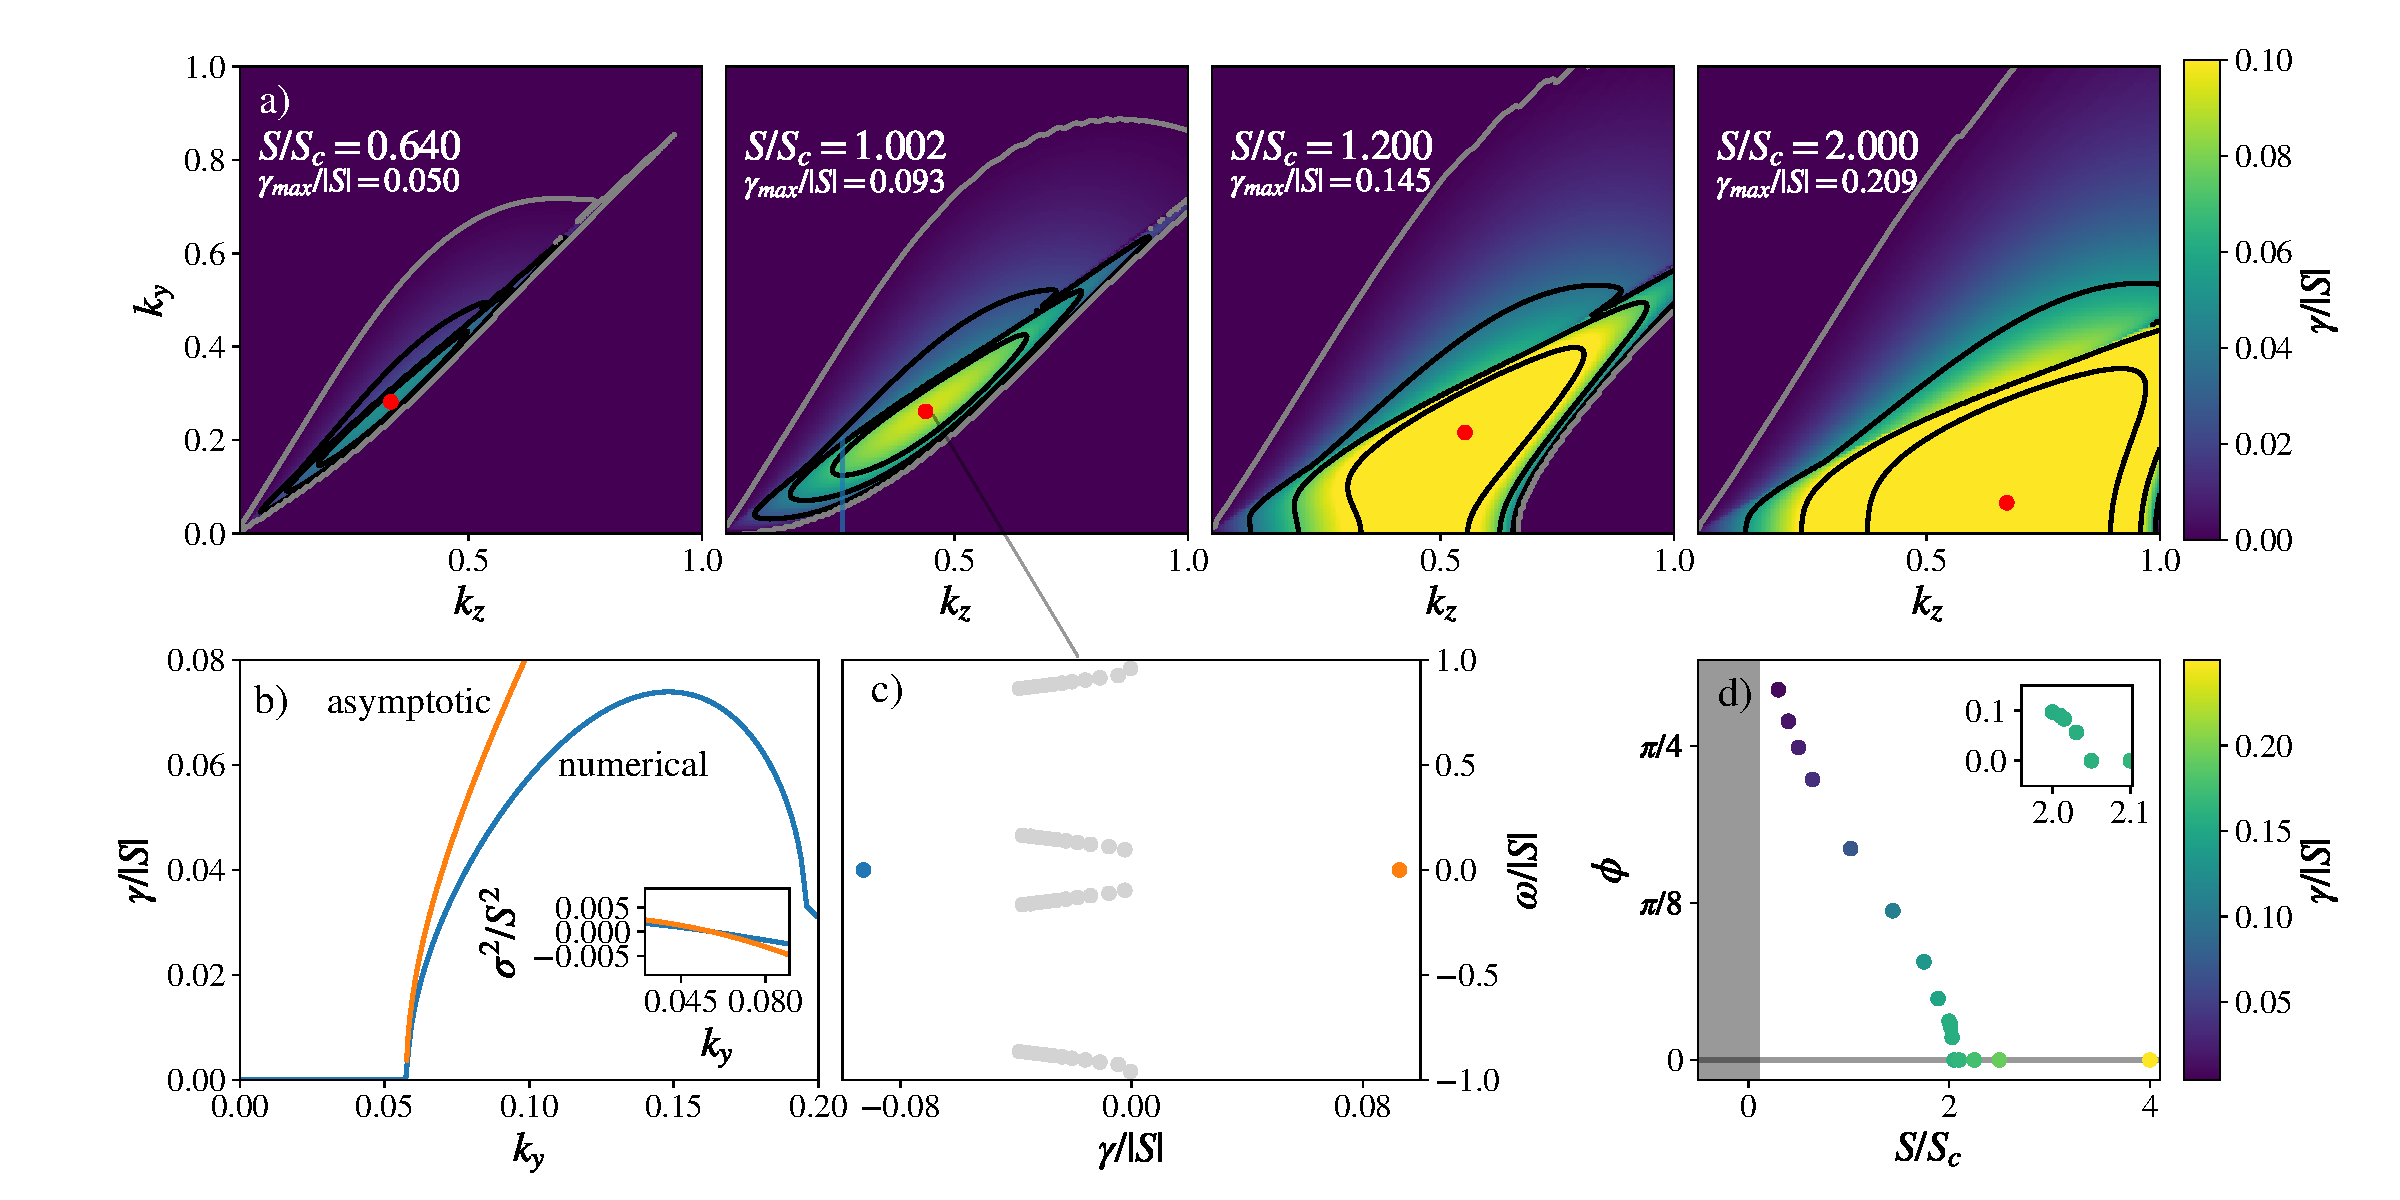
\includegraphics[width=\textwidth]{fig_1.pdf}
  \caption{Growth rates for three-dimensional MRI modes. a) growth rates $\gamma$ over a grid of $k_y$ and $k_z$ for four values of supercriticality $\SSC$. The white contour highlights $\gamma = 0$; the red dots indicate the fastest growing mode. At $\SSC = 0.640$, there are no two dimensional modes. b) Growth rate vs $k_y$ for $k_z = ???$ at $\SSC = 1.002$ (highlighted by the blue line in a). The orange line gives the asymptotic result from equation~(\ref{eq:asymp}) and the blue line are the numerical results. The asymptotic form is valid as $\SSC \to 1$ and $k_y \ll 1$. c) The full discrete spectrum of the MRI for $(k_y, k_z) \simeq (0.263, 0.447)$. The unstable mode is plotted in orange, its stable complex conjugate is blue, and all other modes are gray.}
  \label{fig:growth_rate}
\end{figure*}
%\twocolumngrid
%
Numerical simulations consistently show axisymmetric modes dominating the early evolution of the MRI before breaking down into 3D MHD turbulence \citep{1995ApJ...440..742H,2018ApJ...853..174H,2019ApJS..241...26D}. 
These ``channel modes'' are exact non-linear solutions for $x$-shearing-periodic domains, and can only saturate via parasitic shear instabilities \citep{1994ApJ...432..213G}.
We use impenetrable, stress-free boundary conditions that are more applicable to stellar interiors. 
But even in disks, any kind of finite radial extent will cutoff the unbounded growth of channel modes. 
We reconcile our results with earlier simulations by showing that the MRI indeed prefers two dimensions for the larger values of  criticality found in disk simulations. 
Figure~\ref{fig:phi} shows the phase angle $\phi = \arctan k_y/k_z$ of the fastest growing mode as function of $\SSC$.
Above $\SSC \gtrsim 2.05$ $\phi=0$, indicating that axisymmetric modes have the fastest growth rates.
For the fiducial run in \citet{1996ApJ...464..690H}, $\SSC \simeq 4.84$ (most works use similar values).
Thus, we predict axisymmetric modes should dominate the linear dynamics for parameters studied in prior numerical simulations.
%
\begin{figure}[h!]
  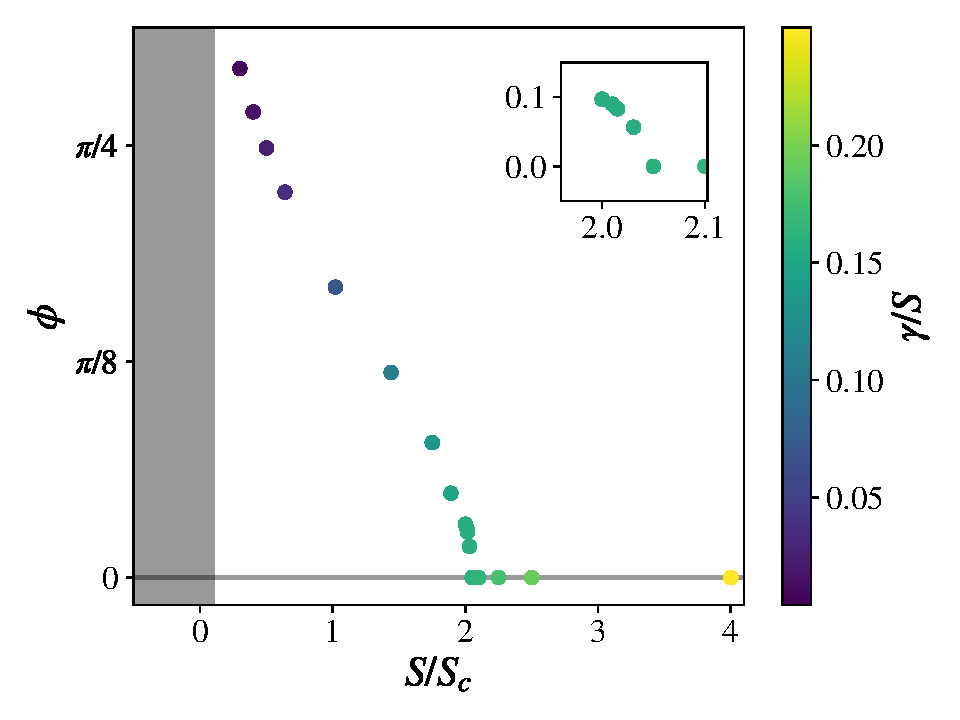
\includegraphics[width=\columnwidth]{phi_vs_ssc_grid.pdf}
  \caption{Angle $\phi$ of mode with respect to $z$ axis vs $\SSC$. The inset shows the transition from axisymmetric modes to three dimensional modes as $\SSC$ decreases below $2.05$. The shaded region indicates stability to all perturbations; the stability limit for three dimensional modes is $\SSC \simeq 0.102$.}
  \label{fig:phi}
\end{figure}
%

Even for $\SSC> 2.05$ there are significant swaths of unstable three-dimensional modes with growth rates comparable to the maximum (figure~\ref{fig:growth_rate}a).
Also, non-normality generically accompanies non-axisymmetry in shearing systems \citep[see][for a discussion relevant to the MRI]{1992MNRAS.255P..25K}.
In non-normal systems, transient amplification can occur for stable modes, and can even cause turbulence.
Therefore significant three dimensionality likely implies important non-normal behavior near onset.

The second implication of the three dimensional modes is of considerably more importance.
These modes produce dynamo action in the linear regime, as evidenced by the presence of non-trivial eigenmodes for all three components of the magnetic field.
This is of considerable significance, as it leads to the possibility of a laminar MRI dynamo operating directly in regions of weak shear.
MRI dynamos have been studied in a number of different contexts \citep{2007PhRvL..98y4502R,2011ApJ...740...18O,2015PhRvL.114h5002S}, but all except one have focused on the turbulent dynamo. The lone exception, \citet{2016MNRAS.462..818B}, is a numerical study that discovered the exponential growth of mean magnetic fields during the linear growth phase of the MRI far from stability.
Our work explains this result in terms of purely linear dynamics:
non-axisymmetric MRI unstable modes drive the exponential growth of magnetic fields.

% \begin{itemize}
% \item non-normal and $k_y$ even when $\phi = 0$ implies important role for linear dynamics at early times. 
% \item Following Squire + Bhattacharjee, this suggests that important stellar layers may in fact be driven by linear dynamics
% \item why is MRI non-oscillatory when hydro shear is oscil or stable?
% \end{itemize}

%If in two-column mode, this environment will change to single-column
% format so that long equations can be displayed. Use
% sparingly.
%\begin{widetext}
% put long equation here
%\end{widetext}

% figures should be put into the text as floats.
% Use the graphics or graphicx packages (distributed with LaTeX2e)
% and the \includegraphics macro defined in those packages.
% See the LaTeX Graphics Companion by Michel Goosens, Sebastian Rahtz,
% and Frank Mittelbach for instance.
%
% Here is an example of the general form of a figure:
% Fill in the caption in the braces of the \caption{} command. Put the label
% that you will use with \ref{} command in the braces of the \label{} command.
% Use the figure* environment if the figure should span across the
% entire page. There is no need to do explicit centering.

% \begin{figure}
% \includegraphics{}%
% \caption{\label{}}
% \end{figure}

% Surround figure environment with turnpage environment for landscape
% figure
% \begin{turnpage}
% \begin{figure}
% \includegraphics{}%
% \caption{\label{}}
% \end{figure}
% \end{turnpage}

% tables should appear as floats within the text
%
% Here is an example of the general form of a table:
% Fill in the caption in the braces of the \caption{} command. Put the label
% that you will use with \ref{} command in the braces of the \label{} command.
% Insert the column specifiers (l, r, c, d, etc.) in the empty braces of the
% \begin{tabular}{} command.
% The ruledtabular enviroment adds doubled rules to table and sets a
% reasonable default table settings.
% Use the table* environment to get a full-width table in two-column
% Add \usepackage{longtable} and the longtable (or longtable*}
% environment for nicely formatted long tables. Or use the the [H]
% placement option to break a long table (with less control than 
% in longtable).
% \begin{table}%[H] add [H] placement to break table across pages
% \caption{\label{}}
% \begin{ruledtabular}
% \begin{tabular}{}
% Lines of table here ending with \\
% \end{tabular}
% \end{ruledtabular}
% \end{table}

% Surround table environment with turnpage environment for landscape
% table
% \begin{turnpage}
% \begin{table}
% \caption{\label{}}
% \begin{ruledtabular}
% \begin{tabular}{}
% \end{tabular}
% \end{ruledtabular}
% \end{table}
% \end{turnpage}

% Specify following sections are appendices. Use \appendix* if there
% only one appendix.
%\appendix
%\section{}

% If you have acknowledgments, this puts in the proper section head.
\begin{acknowledgments}
We would like to thank Steve Tobias for helpful conversations on this work.
JSO acknowledges funding from NASA LWS grant No. NNX16AC92G and Research Corporation Scialog Collaborative Award (TDA) ID\#24231. Computations were performed on the \emph{Leavitt} cluster at the Bates College High Performance Computing Center.
Morgan Baxter acknowledges support from NASA LWS grant No. NNX16AC92G.
\end{acknowledgments}

% Create the reference section using BibTeX:
\bibliography{mri}

\end{document}
%
% ****** End of file apstemplate.tex ******

